%\section{Definition}
% --------------------------------------------------- Slide --
%\subsection{Definition}
\label{definition}
\begin{frame}\frametitle{Definition}
  \begin{definition}
 Let V be a vector space over a field F and let Q be a quadratic form on V
valued in F . The Clifford algebra $Cl(Q)$ is the algebra over F generated by V and defined
by the relations:
\begin{center}
$v_{1} v_{2} + v_{2}v_{1} = 2Q(v_{1} , v_{2} ) . 1$
 
\end{center}

%where 1 is the unit, considered to be the multiplicative unit in the ground field F .
  \end{definition}
  
  
 Particular cases:
 \\
\textbf{Nondegenerate Clifford algebra} $Cl_{p,q}$
\begin{center}
	 $(e_a)^2 = \pm e\: ,\:  e_a e_b = − e_b e_a \: ,\:  a \neq b;$
\end{center}
 \\
 \textbf{Clifford algebra of the Euclidian space $R^n$} : $Cl_n :=Cl_{p,0}$
\begin{center}
	 $(e_a )^2 = e\: ,\:  e_a e_b = −e_b e_a \: ,\:  a \neq b;$
\end{center}
  
 \end{frame} 
 
  
  
  
\begin{frame}\frametitle{Properties of Clifford Algebra} 
\begin{itemize}
	\item 

 Clifford Algebra Combine inner and outer product to defined the geometric product \\
\begin{center}
	$AB = A.B + A \wedge B$
\end{center}
	\item 
 % Unlike the standard vector analysis whose primitives are scalars and vectors for representing points and lines, 
 Clifford Algebra has additional spatial primitives for representing plane and volume segments in two and three dimensions, %and
 	\item 
 It can be extended to any number of higher dimensions :
 %%by the same basic scheme, and they do, with remarkably useful properties.
  
\begin{center}
	scalar , vector , bivector , trivector ....
\end{center}
  
  \end{itemize} 
\end{frame}
  
  
  
  
  
  
  
  
 \begin{frame}\frametitle{Properties of Clifford Algebra} 


 \begin{figure}[t]

	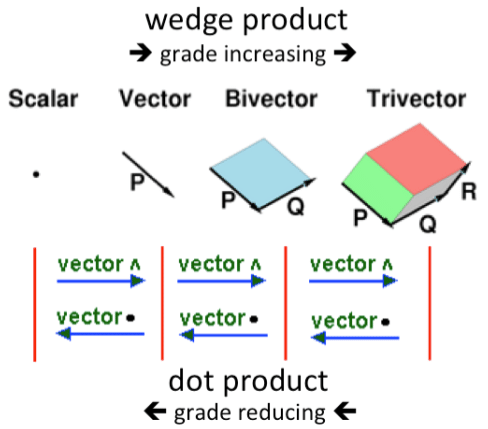
\includegraphics[height=4cm, width=0.7\textwidth]{examples/figures/2.png}
 	\centering
 	 	\caption{Some primitives of Clifford Algebra }
 \end{figure}
 
 
   Clifford Algebra = complex numbers + quaternions + vector analysis + matrix analysis + tensor analysis + spinor algebra ...
   	
\end{frame}


